\documentclass{article}
\usepackage{main}

\title{Dérivation locale et globale}
\author{Terminale STMG2}
\date{}

\begin{document}
\maketitle

\section{Tangente}
\begin{enumerate}
\item Rappeler la définition de tangente à la courbe d'une fonction.

\answersline
\item Représenter la tangente en $0$ de la courbe de la fonction représentée ci-après.
\end{enumerate}

\begin{center}
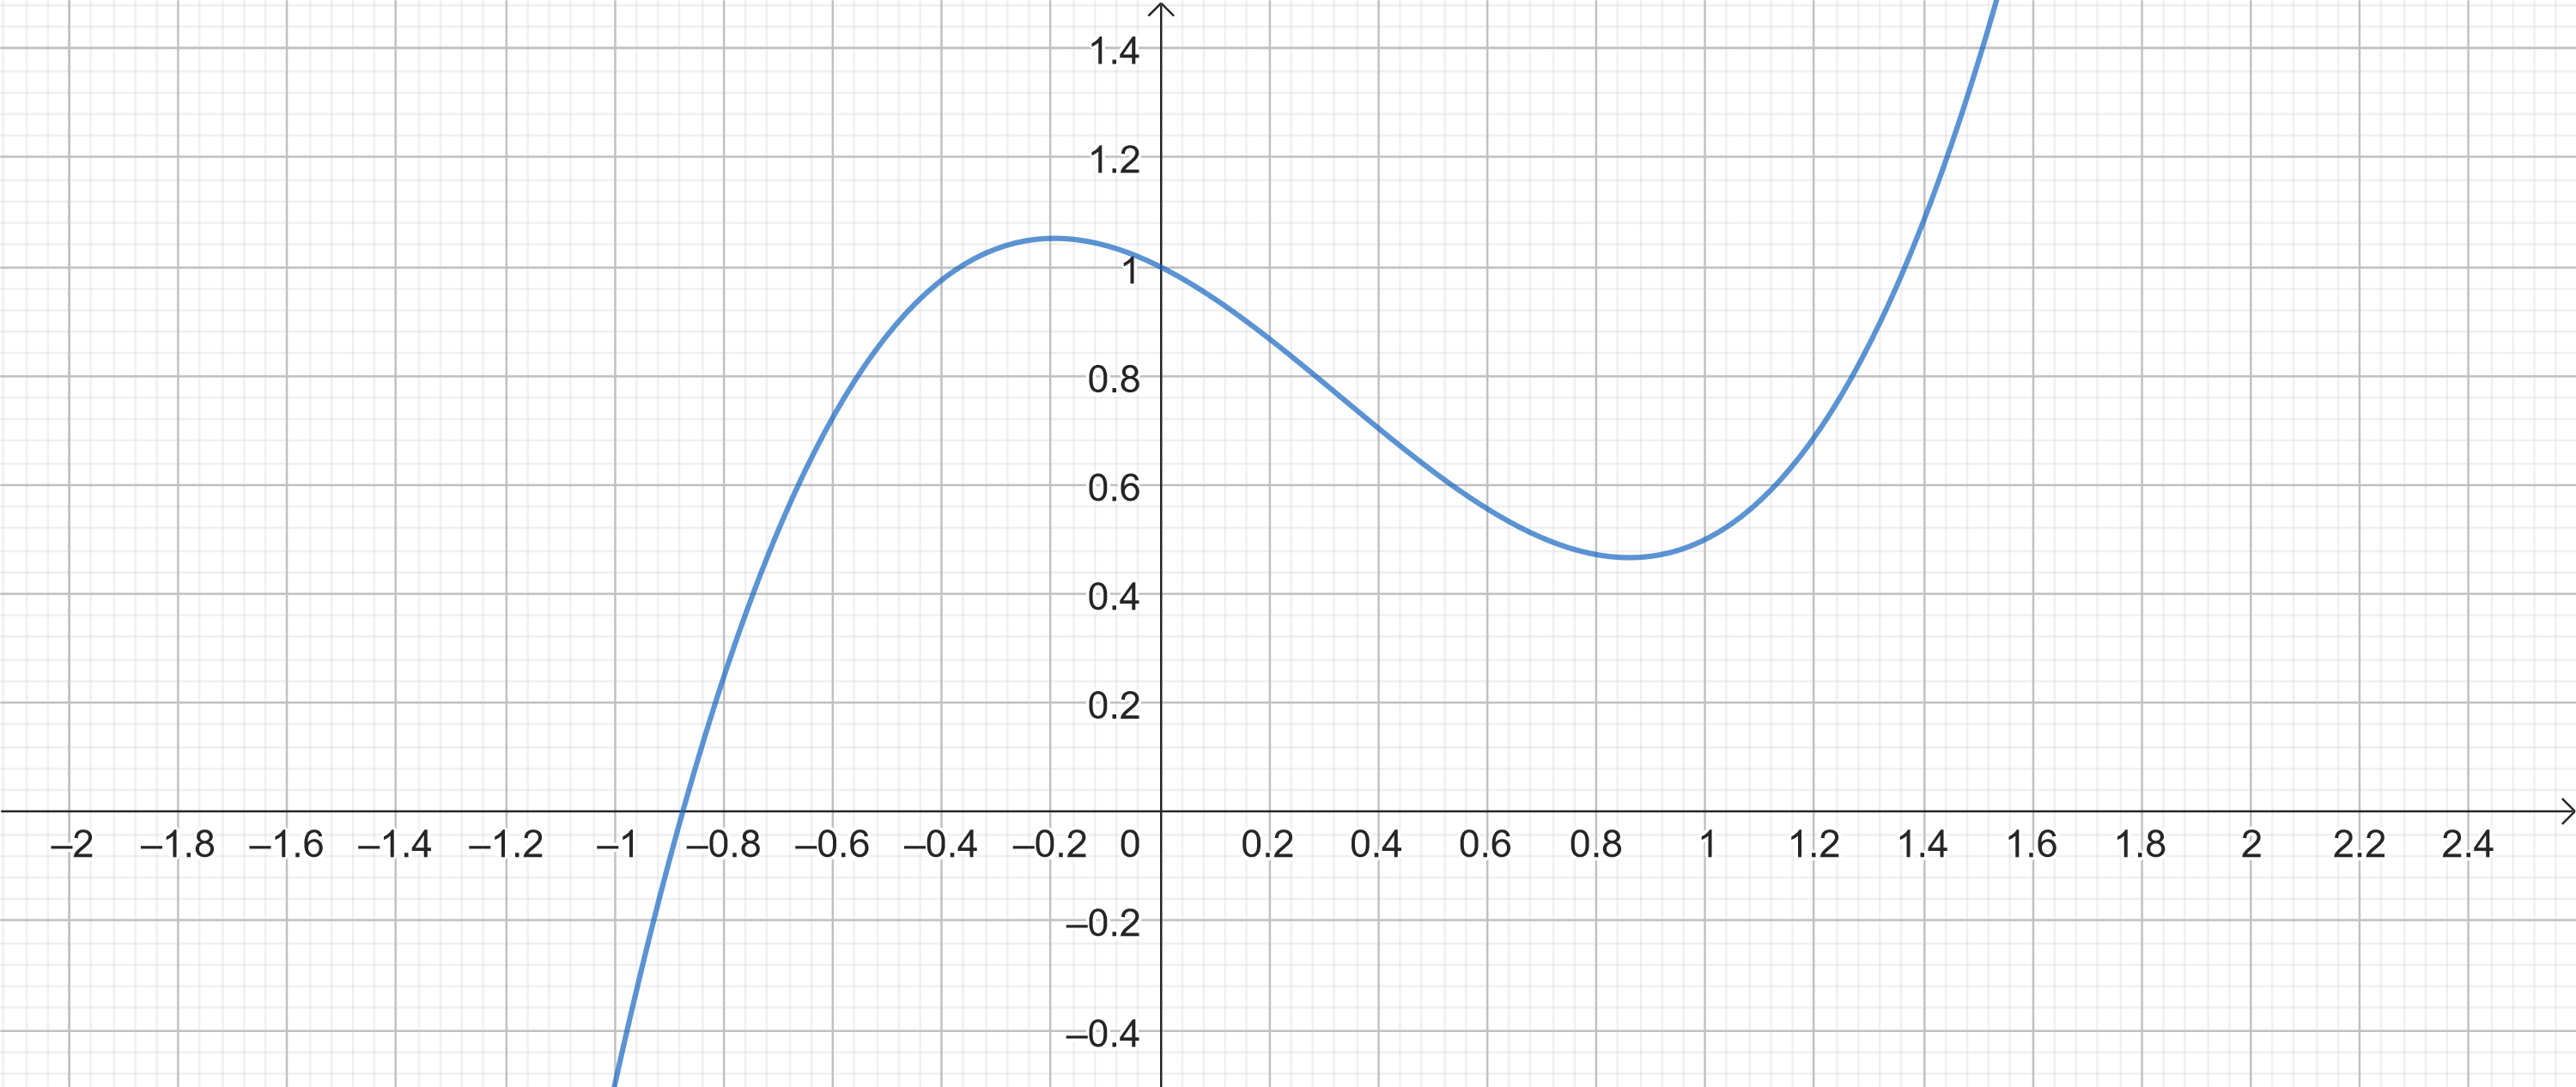
\includegraphics[width=\textwidth]{Courbe_1.png}
\end{center}
\begin{enumerate}[resume]
\item Quelle information nous donne la pente de la tangente que vous venez de représenter ?

\answersline
\end{enumerate}
\begin{tcolorbox}
\begin{definition}
Soit $f$ une fonction, et $a$ un nombre. On suppose que $f$ est définie sur $a$, et que la courbe représentative $\mathcal{C}_f$ admet une tangente en $a$. Alors la pente de cette tangente est appelée \textbf{dérivée de $f$ en $a$}, et notée $f'(a)$.
\end{definition}
\end{tcolorbox}

\section{Fonction dérivée}

Pour chaque point $a$ sur laquelle la courbe $\mathcal{C}_f$ admet une tangente, la tangente présente une pente. On représente ci-après la fonction suivante, qui à chaque $a$ associe la pente correspondante $f'(a)$.

\begin{center}
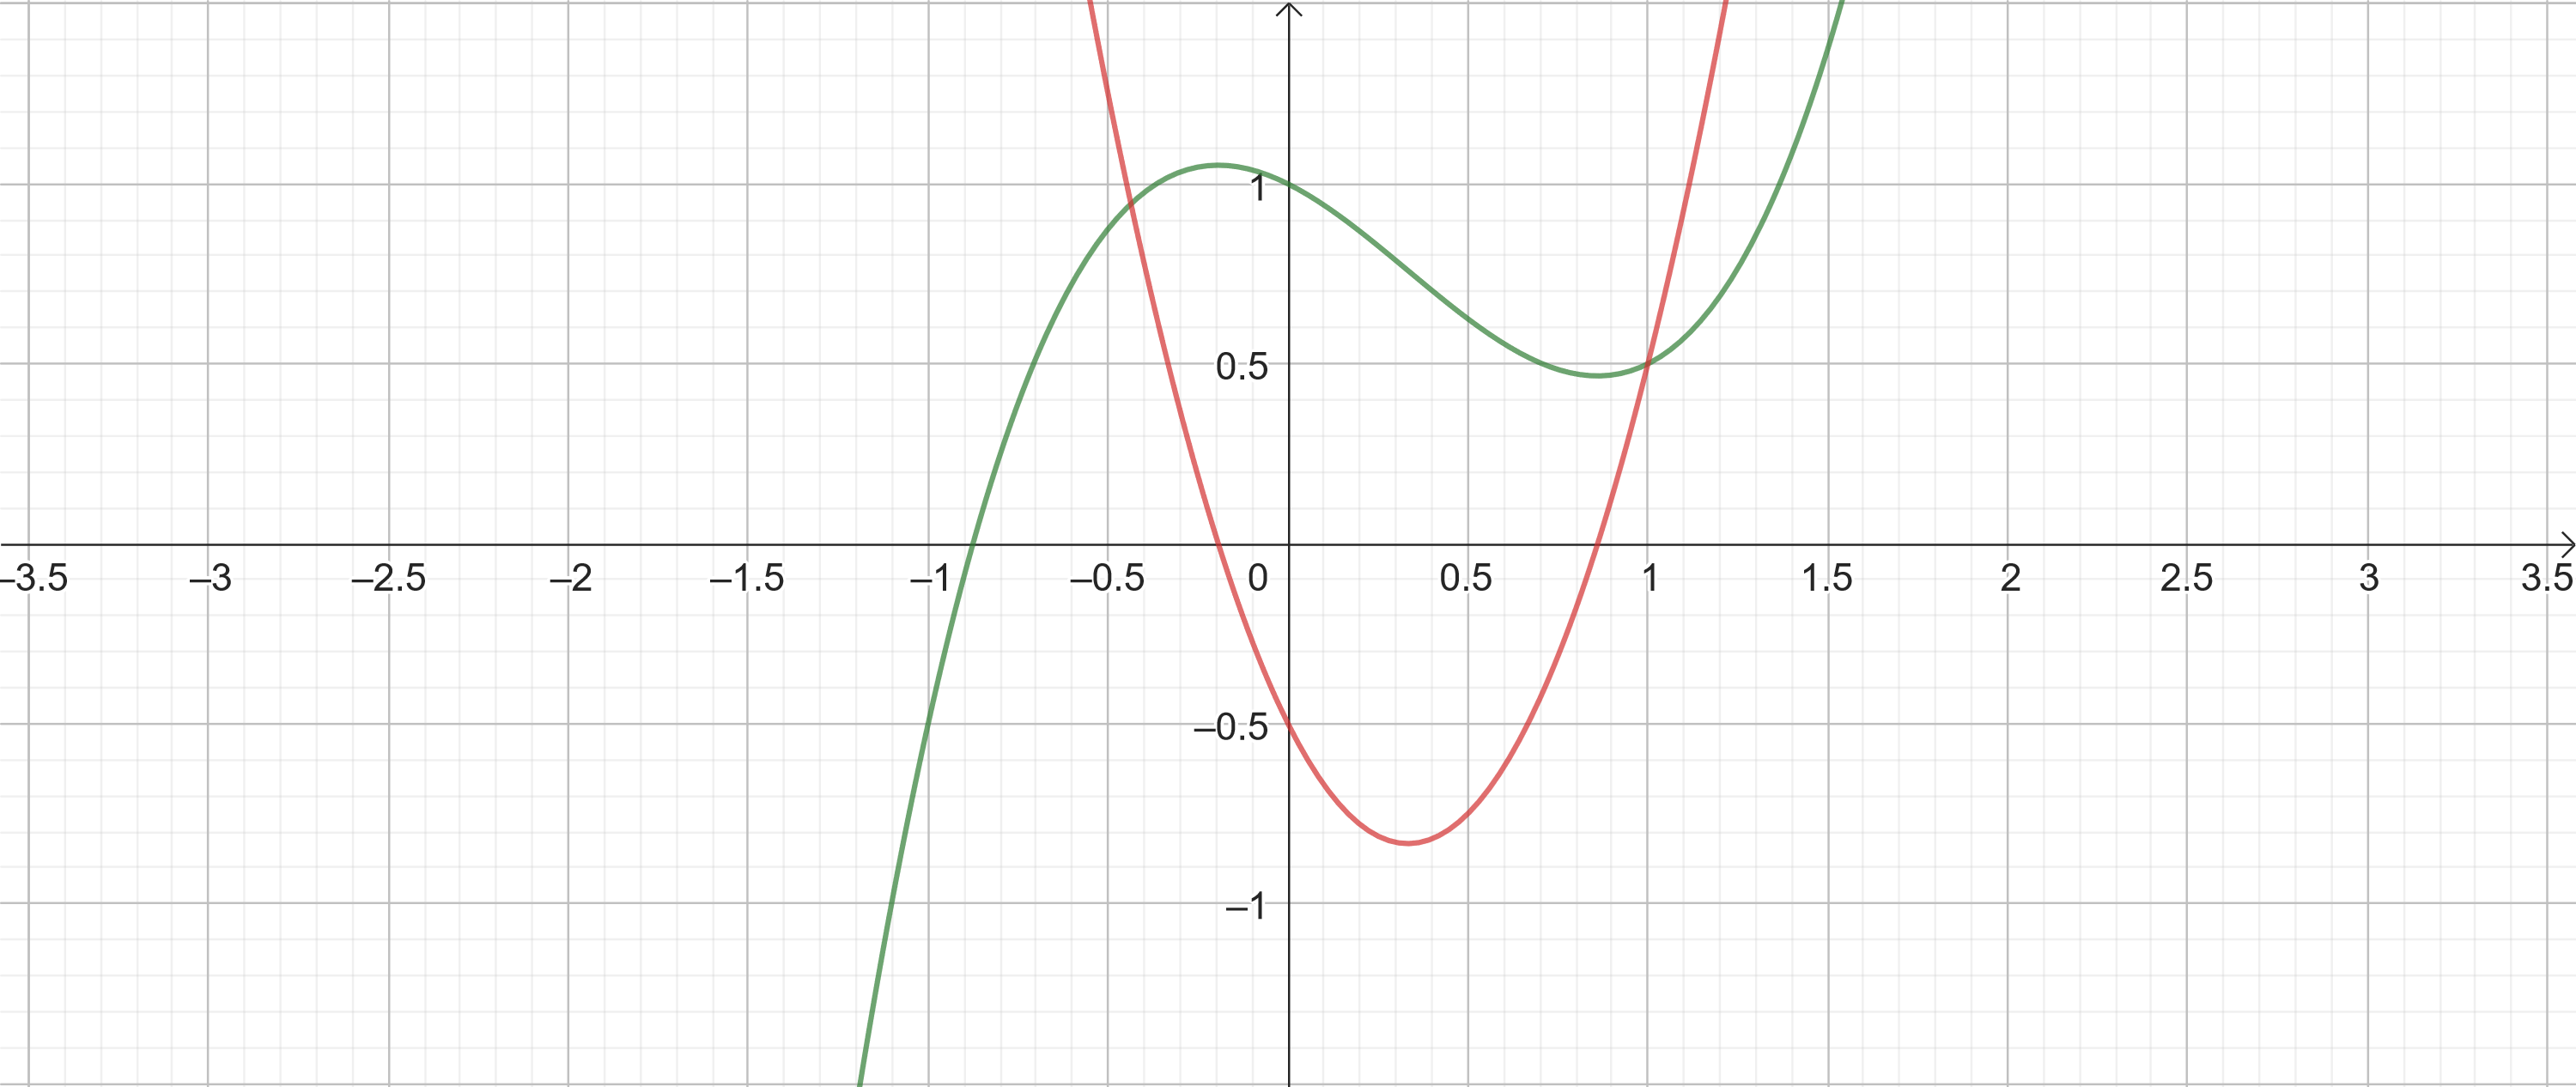
\includegraphics[width=\textwidth]{Courbe_2.png}
\end{center}

\begin{enumerate}
\item Indiquer comment lire cette nouvelle courbe pour en déduire des informations sur la première.

\answersline

\item En déduire précisément sur quel intervalle la fonction $f$ est décroissante.

\answersline
\end{enumerate}

\begin{tcolorbox}
\begin{definition}
Soit $f$ une fonction. On dit que la fonction est \textbf{dérivable sur un ensemble $I$} si sa courbe représentative admet une tangente sur chaque point de $I$.

Dans ce cas, la \textbf{fonction dérivée} de $f$ sur $I$ est la fonction définie sur $I$ qui à chaque nombre $a \in I$ associe la pente de la tangente de $\mathcal{C}_f$ en $a$.
\end{definition}
\end{tcolorbox}
\begin{proposition}
Soit $f$ une fonction dérivable sur un ensemble $I$. Alors $f$ est croissante sur les ensembles où $f'$ est positive, et $f$ est décroissante sur les fonctions où $f$ est négative.
\end{proposition}
\section{Calcul de fonction dérivée}
\begin{tcolorbox}
\begin{proposition}
\hfill

\begin{itemize}
\item La fonction $x \mapsto 1$ est dérivable sur $\R$, et sa dérivée est la fonction $x \mapsto 0$. 
\item La fonction $x \mapsto x$ est dérivable sur $\R$, et sa dérivée est la fonction $x \mapsto 1$. 
\item La fonction $x \mapsto x^2$ est dérivable sur $\R$, et sa dérivée est la fonction $x \mapsto 2x$. 
\item La fonction $x \mapsto x^3$ est dérivable sur $\R$, et sa dérivée est la fonction $x \mapsto 3x^2$. 
\end{itemize}
\end{proposition}
\end{tcolorbox}
\begin{tcolorbox}
\begin{proposition}
\hfill

\begin{itemize}
\item Soit $c$ un nombre reel et une fonction $f$ dérivable sur un ensemble $I$. Alors la fonction $x \mapsto c \times f(x)$ est dérivable sur $I$ de dérivée $x \mapsto c \times f'(x)$.
\item Soient $f$ et $g$ deux fonctions dérivables sur un ensemble $I$. Alors la fonction $x \mapsto f(x) + g(x)$ est dérivable sur $I$ de dérivée $x \mapsto f'(x) + g'(x)$. 
\end{itemize}
\end{proposition}
\end{tcolorbox}
\begin{enumerate}
\item Calculer la dérivée de $g : x \mapsto x^2 - 3x + 1$.

\answersline

\item En déduire le tableau de variation de $g$.
\begin{center}
\begin{tikzpicture}
\tkzTabInit{$x$/1, Signe de $f'(x)$/2, Variations de $f$/2}{$-\infty$,$+\infty$};
\end{tikzpicture}
\end{center}
\item Mêmes questions pour $h : x \mapsto x^2 - 4x - 5$ et $i : x \mapsto -2x^3 - 7x$.
\end{enumerate}
\end{document}